\section{Иерархия}
\label{sec:MCFGHierarchy}
\tikzsetfigurename{MCFG_Hierarchy_}

\mytodo{Свойство поглощения ранга: проверить формулу  (m*(k-1))-MCFL(r-k) subset m-MCFL(r) по Seki1991 -- при k=1 даёт 0-MCFL(r-1), что не определено.}

Для MCFG существует нетривиальная иерархия как по максимальному рангу $m$, так и по максимальной длине правой части $r$.

\begin{theorem}[Иерархия по $m$~\sidecite{SEKI1991191}]
    \label{thm:hierarchy_m}
    Язык $L_{m+1} = \{a_1^n b_1^n \cdots a_{m+1}^n b_{m+1}^n \mid n \in \mathbb{N}\}$ является $(m+1)$-MCFL($1$), но не является $m$-MCFL($r$) ни для какого $r$.
\end{theorem}
\mytodo{Дать формальное определение языка $L_{m+1}$ до его использования в формулировке теоремы.}

\begin{marginfigure}
    \centering
    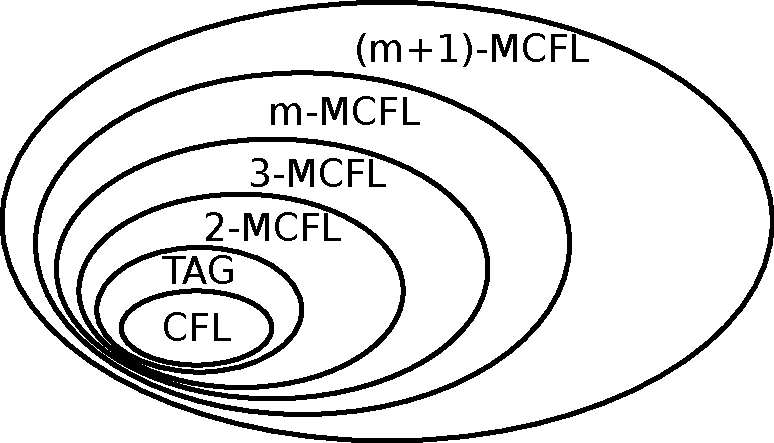
\includegraphics[width=\marginparwidth]{part_02_Foundations/chapter_08_MCFG/figures/mcfg.pdf}
    \caption{Иерархия MCFL по максимальному рангу $m$}
    \label{fig:mcfg_hierarchy_m}
\end{marginfigure}
\mytodo{Перевести PDF-иллюстрации иерархии в TikZ.}

\begin{theorem}[Иерархия по $r$ для $m=1$]
    \label{thm:hierarchy_r_1}
    \begin{enumerate}
        \item $1$-MCFL = CFL.
        \item $1$-MCFL($1$) $\subsetneq$ $1$-MCFL($2$).
        \item $1$-MCFL($r$) = $1$-MCFL($r+1$) для всех $r \ge 2$.
    \end{enumerate}
\end{theorem}

\begin{theorem}[Иерархия по $r$ для $m=2$~\sidecite{rambow1999independent}]
    \label{thm:hierarchy_r_2}
    $2$-MCFL($2$) = $2$-MCFL($3$).
\end{theorem}
\mytodo{Уточнить: верно ли 2-MCFL(1) ⊊ 2-MCFL(2) или 2-MCFL(1) = 2-MCFL(2)?}

\begin{theorem}[Общий случай~\sidecite{SEKI1991191,rambow1999independent}]
    \label{thm:hierarchy_r_general}
    Если $m > 2$ и $r > 2$, то $m$-MCFL($r$) $\subsetneq$ $m$-MCFL($r+1$).
\end{theorem}

\begin{marginfigure}
    \centering
    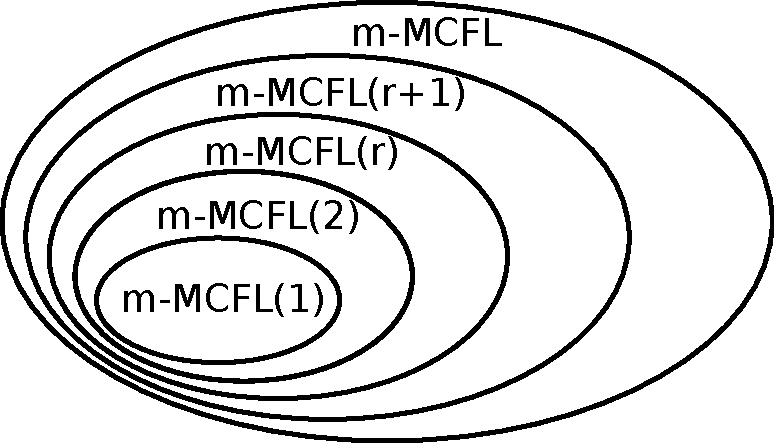
\includegraphics[width=\marginparwidth]{part_02_Foundations/chapter_08_MCFG/figures/mcfg_2.pdf}
    \caption{Иерархия MCFL по максимальной длине правой части $r$}
    \label{fig:mcfg_hierarchy_r}
\end{marginfigure}

Кроме того, известно свойство поглощения ранга: для любых $r \ge 2$ и $k \ge 1$ таких, что $k \le r-2$, имеет место включение
$(m \cdot (k-1))$-MCFL($r-k$) $\subseteq m$-MCFL($r$)~\sidecite{SEKI1991191}.
\mytodo{Добавить сводную таблицу/диаграмму иерархии MCFL по m и r.}
